\documentclass{article}
\usepackage[utf8]{inputenc}
\usepackage[english]{babel}
\usepackage{amsmath}
\usepackage{amssymb}
\usepackage{graphicx}
\usepackage{listings}
\usepackage{color}
\usepackage{amsthm}
\usepackage{babel} 
\graphicspath{ {./images/} }
% \includegraphics{sun}

\newtheorem{theorem}{Theorem}
\newenvironment{amatrix}[1]{%
  \left(\begin{array}{@{}*{#1}{c}|c@{}}
}{%
  \end{array}\right)
}
% \newlist{background}
% \setlist[background]{
%   label = \textbf{Background \arabic*.}, 
%   wide
% }


\renewcommand{\qedsymbol}{Q.E.D.}
\newcommand{\norm}[1]{\left\lVert#1\right\rVert}
\newcommand{\inpro}[2]{\langle#1,#2\rangle}
\newcommand{\proj}[2]{\text{proj}_{#2}\left(#1\right)}

\definecolor{dkgreen}{rgb}{0,0.6,0}
\definecolor{gray}{rgb}{0.5,0.5,0.5}
\definecolor{mauve}{rgb}{0.58,0,0.82}
\lstset{frame=tb,
  language=Java,
  aboveskip=3mm,
  belowskip=3mm,
  showstringspaces=false,
  columns=flexible,
  basicstyle={\small\ttfamily},
  numbers=none,
  numberstyle=\tiny\color{gray},
  keywordstyle=\color{blue},
  commentstyle=\color{dkgreen},
  stringstyle=\color{mauve},
  breaklines=true,
  breakatwhitespace=true,
  tabsize=3
}

\title{CS 241 Final Project: MOBA Wave Management}
\author{Christian Gutierrez}
\date{Spring 2022}

\begin{document}

\maketitle

\newpage
\section{Background}
Videogames have become an increasingly popular hobby amongst most people, and its no secret as a segment called “eSports” has developed into an approximately 1 billion dollar industry. Within eSports, many different “Sports” (videogames) reside within the wide genre. The most popular belonging to the MOBA (Multiplayer Online Battle Arena) genre which pits two teams (typically of 5 players) to take over and destroy each other’s base in order to achieve victory. For the context of this paper, we will be referring to the most popular game in the MOBA genre being “League of Legends”. The primary objective of the game is to level up and empower your character(champion) to destroy turrets that defend the enemy base. After destroying all the turrets in a section(lane) the core of the base(nexus) is exposed, allowing that team to destroy it and achieve victory. There are various nuances to the game such as the different positions of Top (typically a tough melee champion), Mid (Mages or melee assassins), Bot (long range “gun” champions with high damage per second) which consist of each lane to each champion; there are also side lane roles like Jungle (mix of champions with high engage potential) and Support (helps the Bot player safely engage the enemy team). While these descriptions are very general to the seasoned player, it will suffice for the context of this paper. Each player in main roles have control over their lane. Throughout the game, tiny soldiers known as minions (or creeps) come in waves of 6 or 7 down each lane and clash to the enemy team’s minions. Players in these lanes can kill these minions to gain gold and experience to level up their champion and increase their power with items purchased. While on a surface level, the strategy most people would think is simple: hit and kill the enemy minions faster to get gold and destroy the enemy turret; however, the answer to more seasoned players is much more nuanced. There are many strategies used to change the overall state of the group of minions called “wave management” used by players where given some initial minion wave state, it can be manipulated with damaging it, changing minion targeting, or letting the wave sit. These actions can influence the minion wave’s position and number of minions given enough time and cycles of new minions arriving to fight. Generally, there are 3 types of waves, pushing, pulling and freezing(neutral). These states change where the “crash point” of the upcoming wave will occur and if the push/pull will be further accelerated given no player influence. In the results section of this paper, we will be showing the results from various initial conditions; what actions will have on the wave and how to best use them to gain an advantage over a lane opponent.
\newpage
\section{Results}
\begin{table}[h]
In order to test the hypothesis in which; given a lane state, can the future position of the wave be predicted. To first test this hypothesis, we must run trials on an unaffected lane to see how long It would take for a wave to crash into the opposing team’s turret. I have conducted several trials in a custom game environment where given normal minion level growth starting at level 1, how will the minions interact and where the lane would go. In the trials I preformed, the minions consistently crashed from the red side and on the 3rd wave. For this paper we can assume that minions have consistent targeting and RNG from minion targeting can be relatively ignored due to its minimal impact on the overall lane. 
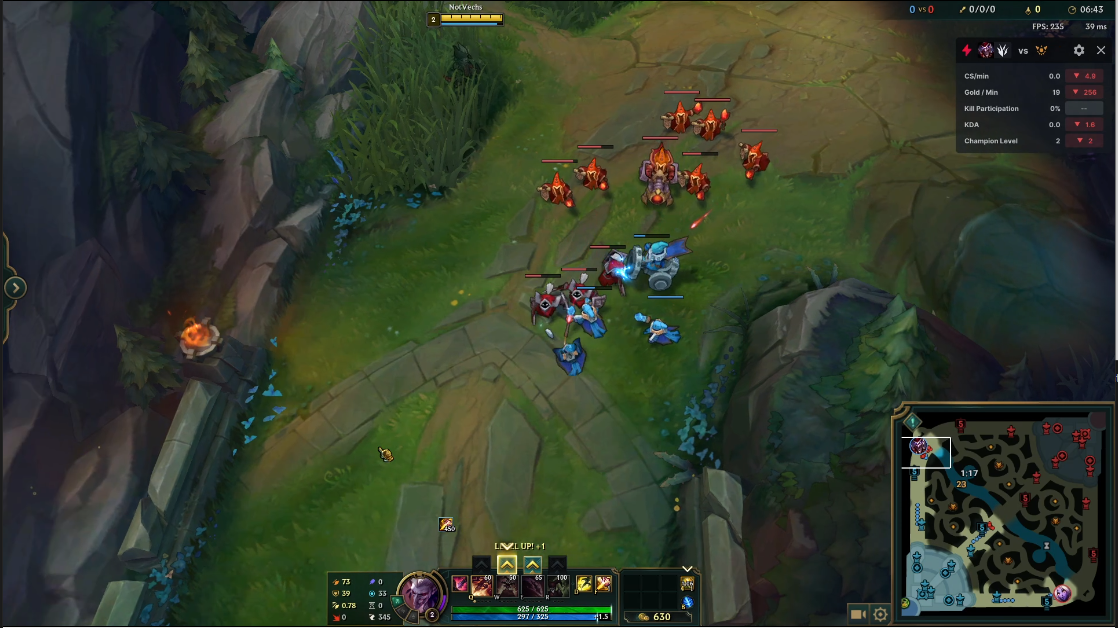
\includegraphics[width=\textwidth]{Crash.PNG}
\caption[Minion Wave Crashing to Blue Side Turret]{Minion Wave Crashing to Blue Side Turret, Wave 3}
\end{table}
To further explore the topic of wave influence, there are several other trials that can be done to affect the wave and see where it goes. In the table below, I have listed several trials that would demonstrate that when affecting the wave in various conditions, how much would it have an effect on it.
\begin{center}
\begin{tabular}{ c c c}
  Level 1 & No Influence & 3 Waves Red Crash\\ 
  Level 1 & 100 Damge to  a Melee Minion & ---\\  
  Level 1 & 200 Damge to  a Melee Minion & ---\\  
  Level 1 & Remove A Minion & ---\\  
  Level 1 & Using the Technique of "Pulling The Wave"  & ---\\
  Level 6 & No Influence  & ---
\end{tabular}
\newpage
\end{center}
After spending some time in the custom environment, the various conditions were tested, and the results are listed below. I personally would have liked to also consider having additional levels and their impact on the speed of lane pushing. It would have taken considerable time, and the results from the only 1 trial conducted at a level starting not from 1 roughly can be extrapolated to potentially more levels for the nuances.
\begin{center}
\begin{tabular}{ c c c}
  Level 1 & No Influence & 3 Waves Red Crash\\ 
  Level 1 & ~100 Damge to  a Melee Minion & 4 Waves Blue Crash\\  
  Level 1 & ~200 Damge to  a Melee Minion & 4 Waves Blue Crash\\  
  Level 1 & Remove A Minion & 2 Waves Blue Crash\\  
  Level 1 & Using the Technique of "Pulling The Wave"  & 5 Waves Red Crash\\
  Level 6 & No Influence  & 3 Waves Red Crash
\end{tabular}
\end{center}
In the end the various wave techniques have demonstrated various changes in the outcome of the wave compared to not influencing the minions. One particular result that confused me was when “Pulling the Wave”, the objective of preforming it is to create a slow push into your side by adjusting the minion targeting to focus one minion at a time. This will result in a safer position compared to a neutral wave state. However, it caused the Red side minions to take even longer to crash into the turret. Possibly this could be due to the influence of minion RNG, but more testing can delve deeper into the subject.
\textit{Recorded Trials can be found at \\https://drive.google.com/drive/folders/1QYnxoKPp4oxKwOXrMW9Sc7SYKZ\\z9mZaT?usp=sharing}
\begin{table}[h]
  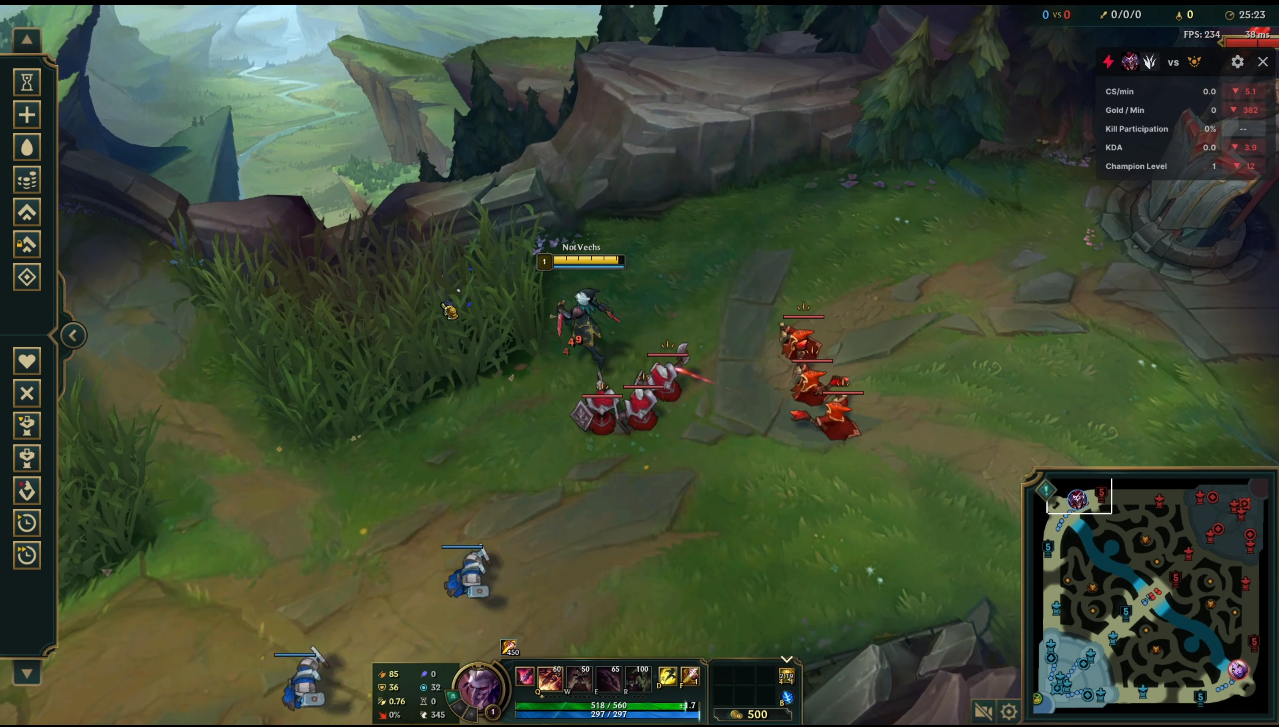
\includegraphics[width=\textwidth]{PullingTheWave.PNG}
  \caption[Pulling the Wave]{Using the Technique of "Pulling the Wave"}
  \end{table}

\newpage
\section{Summary}
The information gathered here is mostly known by higher level players that seek to play this game in a highly competitive fashion. While not exclusively reserved for elite ELO players, you too can use these techniques to gain an advantage over your enemy. For example, given a jungle player with standard pathing, you can expect them to try to contest the scuttle crab at around 3:00, and heading to bot lane at around 3:20. With the information of various initial wave adjustments, you can best set yourself up to either defend against the enemy jungle ganking your lane or prepare your lane so it is easier for your jungle or ally player to assist you in winning lane. However, when it comes to predicting where your lane will land is mostly a trick of eyeballing how much damage is needed for the lane to move in the desired direction. In the final section of this paper, we will take a deeper dive into potentially creating a formula where given some initial wave health, how would the lane push or pull and how long until the desired conditions are met.


% \newpage
\section{"Playing" with the Results}
Using the information gathered earlier, there seems to be potentially further analysis we can apply to the given information. Damaging a wave can have impacts if done in the correct amounts, and generally minion targeting RNG seems to be a minor factor ignoring neutral wave states. With this, I have devised a very simple formula to attempt to determine how using carryover minions from previous waves and players damaging minions to try to get a model of where a wave will land.\\
\begin{equation}
  \sum_{0}^{z}{(H_{e}+D_{e}) - (H_{a}+D_{a}) \pm H_{extra} * K}
\end{equation}
Given $z$ is number of waves calculated; $H$ for hitpoints of each wave (ally and enemy and extra per side); $D$ for damage each wave (ally and enemy); $K$ for minion pushing constant.\\
While the above model is not perfect, and K is dependent on each wave and minion targeting, it is easier to simplify the state of the wave with an absolute number. Given more time and research, potentially a K number to accurately describe the potential of the wave in a very strong case. While arguably it would be impossible to distill various factors like minion targeting to a simple number, it is arguably accurate for the scenario. Another pitfall of distilling the entire wave to just HP of the carry over wave, it is ignoring the type of minions alive. It could be made more accurate to the HP’s of melee, caster and cannon minions. This would cause undue confusion that this model is attempting to simplify.\\
\begin{table}[h]
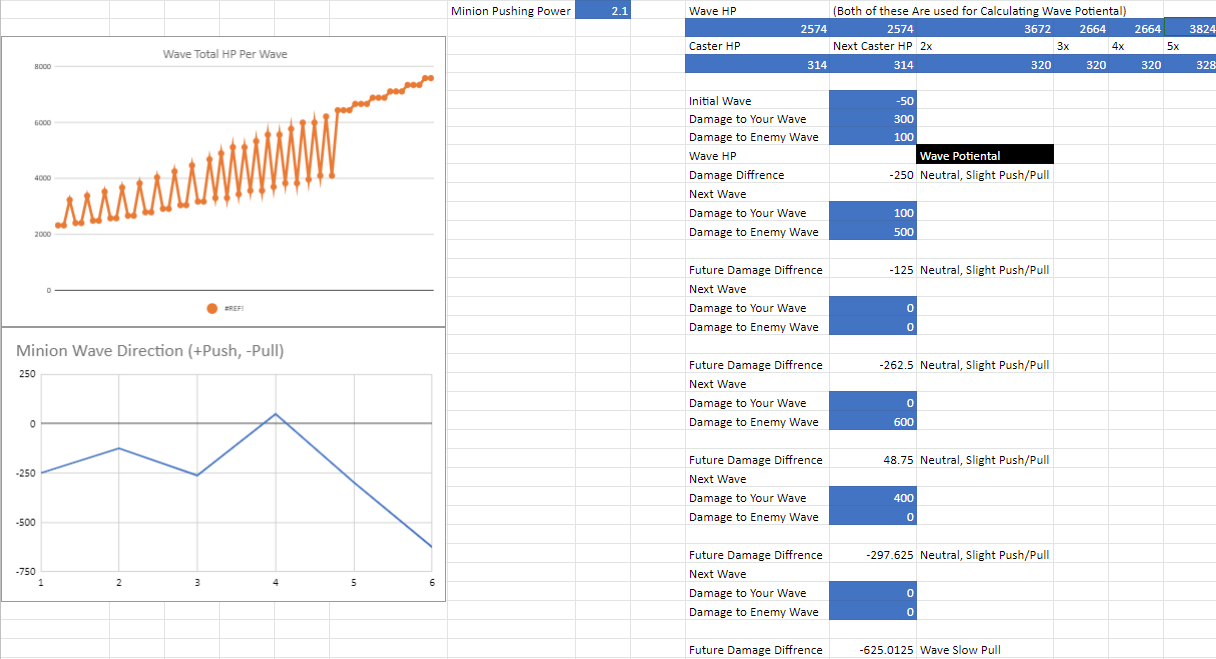
\includegraphics[width=\textwidth]{WaveCalc.PNG}
\caption[Spreadsheet]{Spreadsheet Used with Test Data, Try it Out!}
\end{table}
I have also created a spreadsheet where you can mess around with various minion conditions and changes to the wave in an emulation of what a wave state will be with a graph clearly showing the movement of the wave. 
\textit{
  \\https://docs.google.com/spreadsheets/d/1cgwxDittMwNl9EIxlo4bZWIxIlmelYz\\MTh4pUQhSjdU/edit\#gid=546790742
}
While the model devised earlier is not perfect, and as a result this spreadsheet, it gives a close enough glance at the movement of waves given some initial conditions.


\end{document}